% !TeX root = ta.tex
\cleardoublepage % memastikan bab baru dimulai di halaman ganjil (kanan)
% ==========================================
% BAB I PENDAHULUAN
% ==========================================
\chapter{PENDAHULUAN}
\label{chap:pendahuluan}
% Latar Belakang
\section{Latar Belakang}
Berdasarkan data \textcite{owid2025causesofdeath} yang dapat dilihat pada Gambar \ref{gambar:causeofdeath}, kanker atau tumor ganas menempati urutan kedua sebagai penyebab kematian tertinggi di dunia setelah penyakit kardiovaskular, dengan perkiraan angka kematian mencapai 10,6 juta jiwa. Di dalam kelompok penyakit mematikan tersebut, tumor otak menjadi salah satu tantangan terbesar dalam dunia kesehatan global. Menurut \textcite{ferlay2024gco1}, terdapat 321.731 kasus baru tumor otak di seluruh dunia, dengan angka kematian mencapai 248.500 kasus. Hal ini menempatkan tumor otak pada peringkat ke-19 dalam jumlah kejadian dan peringkat ke-12 dalam jumlah kematian. Berdasarkan data tersebut, perbandingan antara peringkat jumlah kejadian dan peringkat jumlah kematian pada tumor selain otak tidak berbeda jauh dibandingkan dengan tumor otak. Perbedaan peringkat antara jumlah kejadian dengan jumlah kematian tumor otak ini menunjukkan urgensi diagnosis tumor otak lebih tinggi dibandingkan tumor yang lain.

\begin{figure}[h]
	\centering
	\captionsetup{justification=centering}
	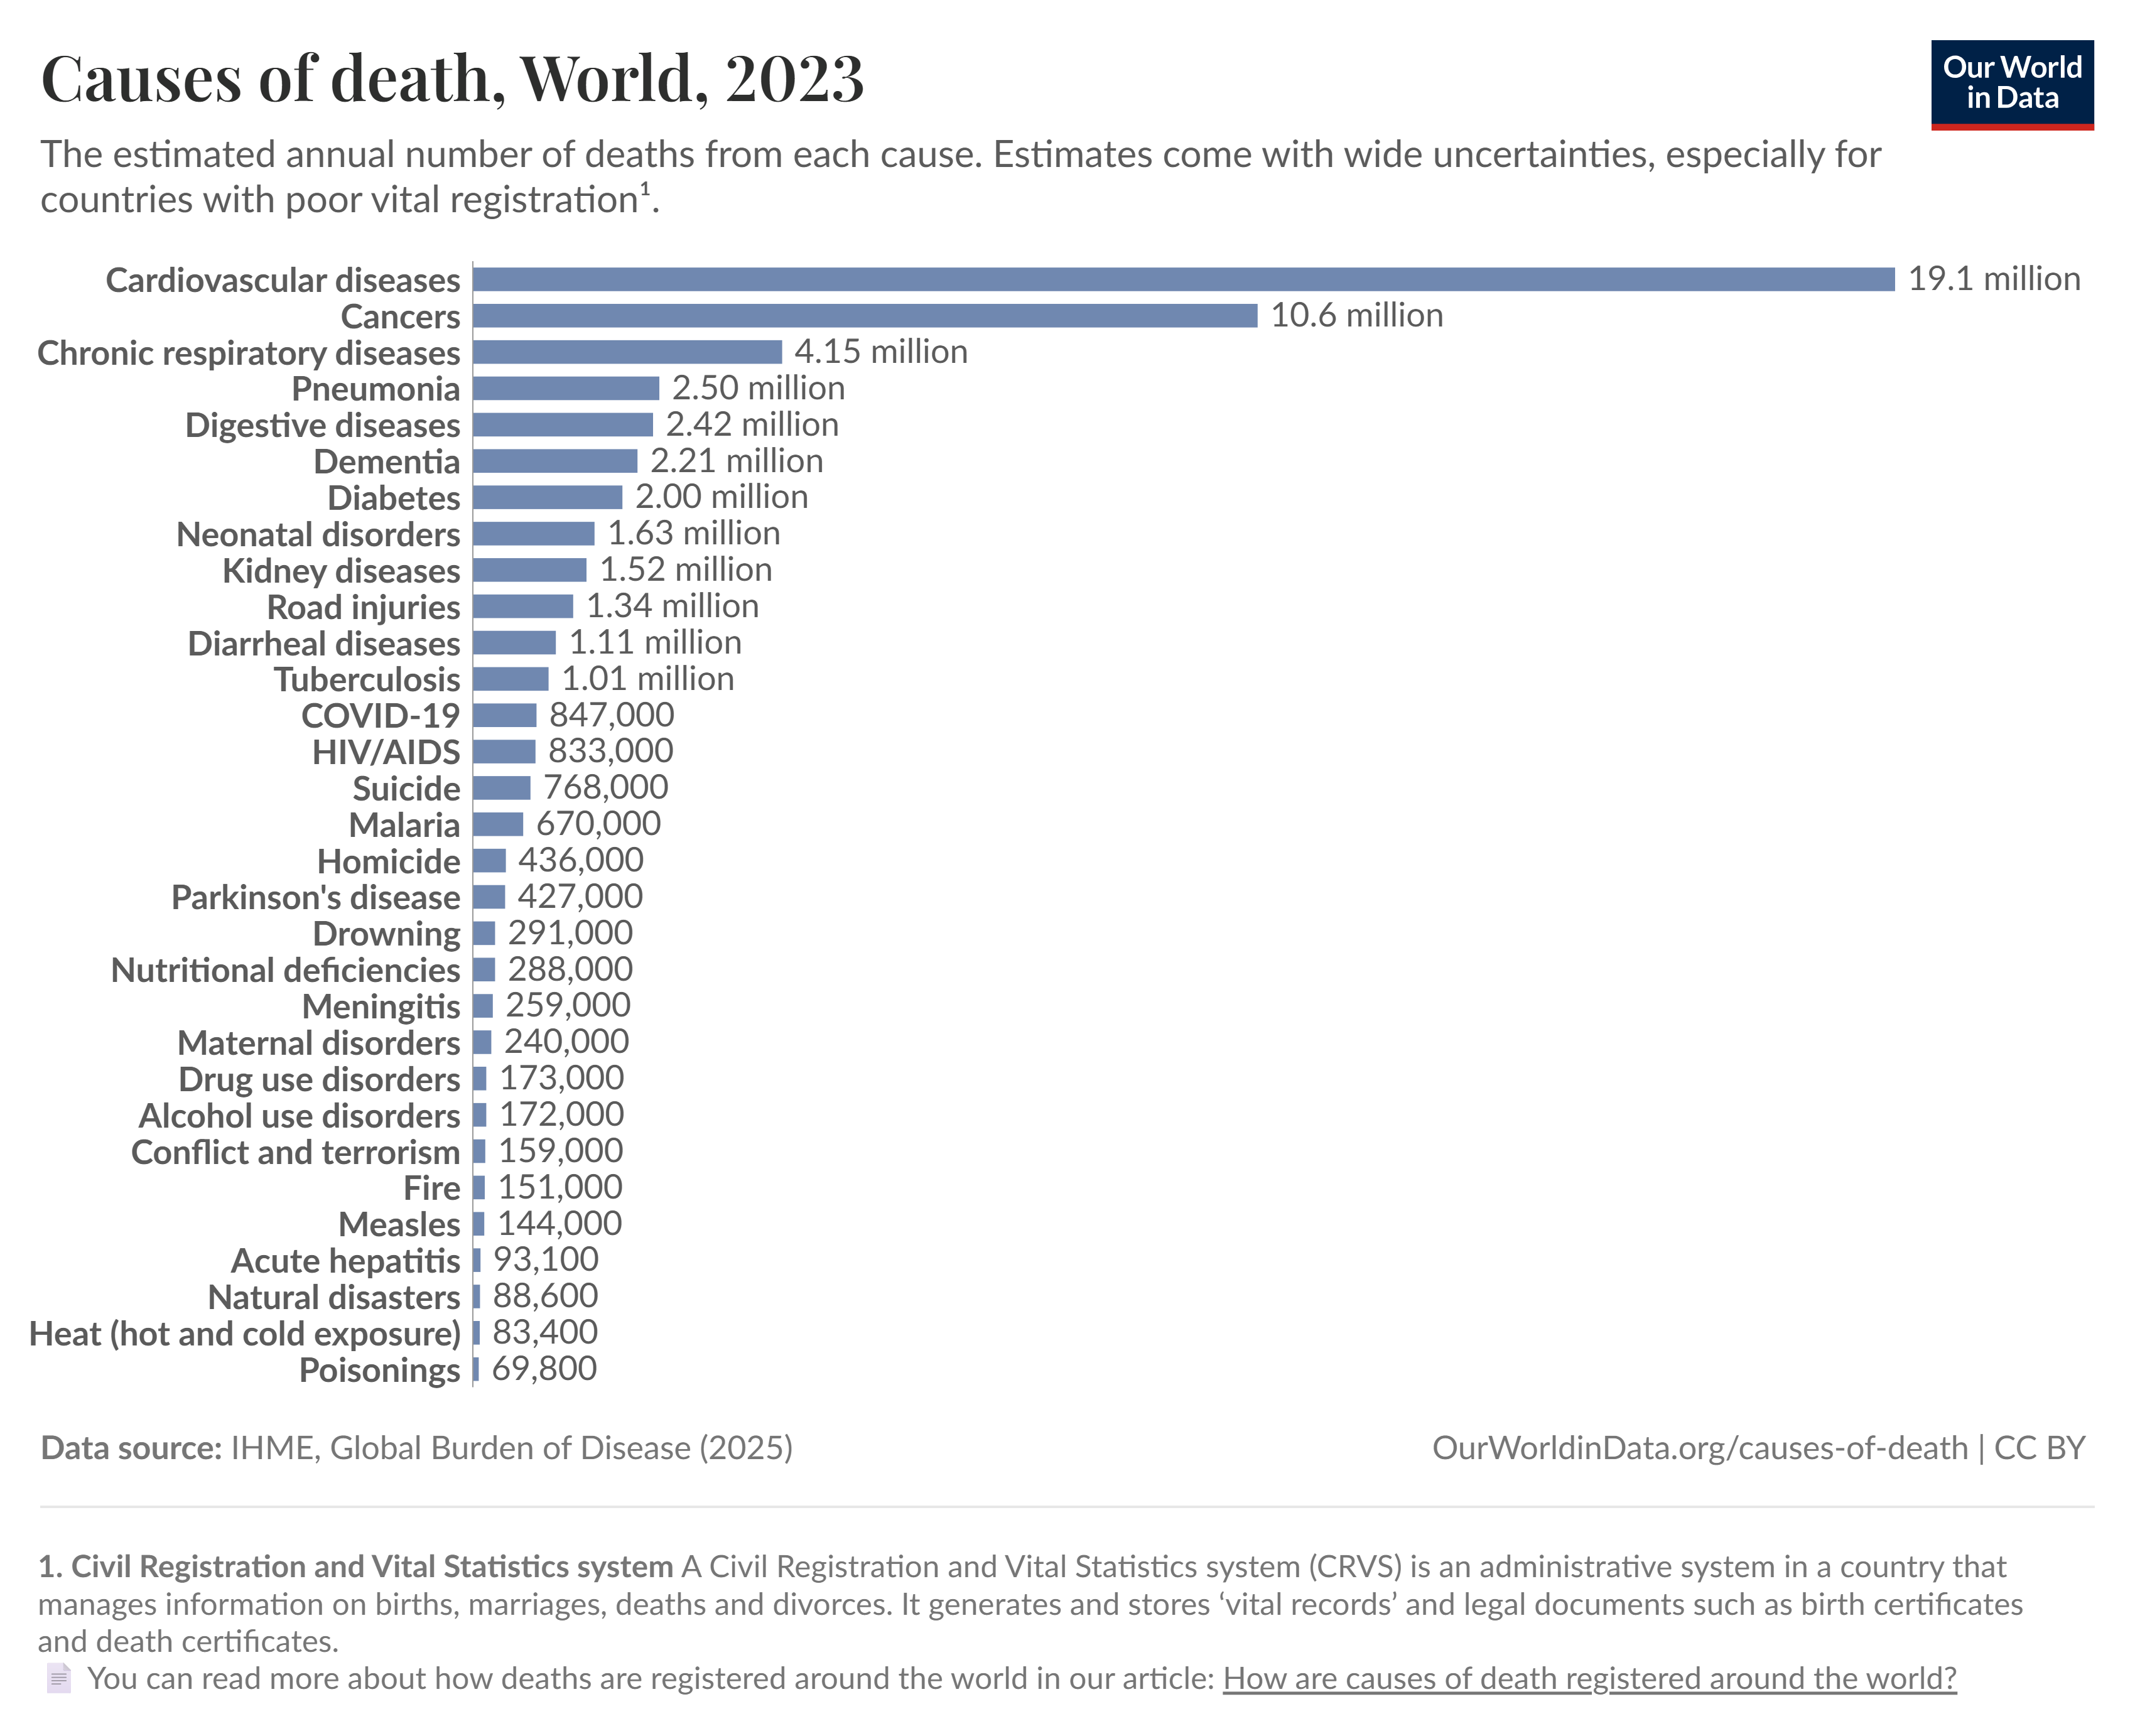
\includegraphics[width=0.7\textwidth]{images/CauseOfDeath.png}
	\caption{Penyebab kematian di dunia tahun 2023 
		\autocite{owid2025causesofdeath}}
	\label{gambar:causeofdeath}
\end{figure}

Di Indonesia, kasus baru tumor otak tercatat sebanyak 5.738 kasus (1,4\% dari total kasus kanker), dengan angka kematian mencapai 5.259 kasus (2,2\%). Hal ini menempatkan tumor otak pada peringkat ke-15 dalam jumlah kejadian dan peringkat ke-11 dalam jumlah kematian. Selain itu, prevalensi lima tahun dari tumor otak mencapai angka 20.134 atau setara dengan 7,7 per 100.000 penduduk \cite{ferlay2024gco2}. Hal ini mengindikasikan hanya sedikit orang yang masih hidup setelah lima tahun didiagnosis menderita tumor otak. Oleh karena itu, pendeteksian dini tumor otak merupakan hal yang krusial untuk keberhasilan pengobatan dan prognosis pasien \cite{kemkes2025tatalaksana}.

Menurut \textcite{mayoclinic2019braintumor}, untuk melakukan diagnosis tumor otak, diperlukan pemeriksaan neurologis, seperti pemeriksaan penglihatan, pendengaran, keseimbangan, koordinasi, kekuatan, dan refleks. Jika terdapat masalah di satu atau lebih area, ini adalah petunjuk untuk melakukan pencitraan medis untuk melihat kondisi lebih lanjut. Terdapat cara yang dapat dilakukan untuk melakukan pencitraan medis pada tumor otak, yaitu pemindaian \textit{CT Scan}, pemindaian MRI otak, dan pemindaian \textit{Positron Emission Tomography} (PET) otak. Oleh karena itu, pencitraan medis merupakan hal yang penting dalam pendeteksian tumor otak. Dari pencitraan medis tersebut, MRI menunjukkan akurasi diagnostik yang lebih tinggi dibandingkan \textit{CT Scan}, yaitu MRI mendeteksi tumor otak pada 60\% kasus dibandingkan dengan 50\% oleh \textit{CT Scan}. MRI menunjukkan akurasi diagnostik yang lebih tinggi, terutama untuk lokalisasi lesi dan penilaian parenkim, memperkuat statusnya sebagai standar emas dalam pencitraan tumor otak \cite{jaffar2025comparative}.

Berdasarkan \textcite{medtech2020hospitalintelligence}, pada tahun 2019, Indonesia memiliki sekitar 750 pemindai \textit{CT Scan} dan pemindai MRI yang jauh lebih rendah di antara 2.764 rumah sakit. Selain itu, disparitas MRI yang ada di Indonesia juga sangat besar. Berdasarkan data pada 2023, Kalimantan Barat hanya memiliki dua sistem MRI dengan jumlah penduduk mencapai lima juta jiwa. Sumatera Barat dengan 5,5 juta penduduk hanya memiliki empat alat kesehatan tersebut \cite{purnama2025disparitas}. Penggunaan MRI juga memiliki ketergantungan terhadap helium. Saat ini, terdapat kelangkaan helium secara global yang berdampak nyata pada penggunaan MRI Indonesia. Saat ini, Indonesia sedang mengembangkan inovasi teknologi MRI dengan desain tanpa helium. Namun, teknologi tersebut masih dalam tahap pengembangan dan belum terbukti dapat menyelesaikan permasalahan kelangkaan MRI di Indonesia \cite{permana2025kelangkaan}. Oleh karena itu, pendeteksian tumor otak melalui MRI sulit untuk dilakukan di Indonesia dan salah satu alat pendeteksian tumor otak alternatif yang sudah lebih banyak digunakan adalah \textit{CT Scan}. Sebuah studi dari \textcite{budiman2024effectiveness} mengonfirmasi bahwa penggunaan \textit{CT Scan} terbukti sangat efektif dan memberikan dampak positif yang signifikan untuk keperluan deteksi dini tumor otak pada manusia.

Aspek yang penting dalam pendeteksian tumor otak adalah diagnosis yang dilakukan oleh radiolog. Menurut \textcite{nuraini2024kesulitan}, Indonesia memiliki kesulitan akses tenaga radiolog dikarenakan distribusi tenaga medis yang tidak merata. Selain itu, diagnosis yang sering kali menghadapi tantangan dalam hal jumlah tenaga yang memadai untuk memenuhi kebutuhan pemeriksaan pasien yang semakin meningkat. Dengan meningkatnya jumlah kasus medis dan populasi yang terus bertumbuh, jumlah tenaga radiolog yang ada saat ini masih belum cukup untuk memenuhi seluruh permintaan pemeriksaan dengan akurat dan tepat waktu.

Saat ini, salah satu solusi yang ditawarkan untuk mengatasi permasalahan deteksi tumor otak adalah menggunakan teknologi \textit{Artificial Intelligence} (AI). Pada penelitian yang dilakukan oleh \textcite{darmiati2023impact}, terdapat hasil bahwa bantuan AI secara signifikan meningkatkan sensitivitas dan spesifisitas semua radiolog dalam pendeteksian tumor pada payudara, dengan peningkatan median masing-masing sebesar 19,4\% dan 12,1\%. Penerapan AI secara langsung dalam praktik klinis juga telah dibuktikan keberhasilannya pada penanganan kasus tumor otak.

Salah satu penelitian terkini yang berfokus pada optimalisasi deteksi tumor otak menggunakan \textit{CT Scan} adalah pengembangan \textit{Correlation Learning Mechanism} oleh \textcite{wozniak2021deep}. Metode ini mengusulkan mekanisme pembelajaran korelasi baru untuk arsitektur jaringan saraf dalam yang menggabungkan \textit{Convolutional Neural Network} (CNN) dengan arsitektur klasik. Hasil penelitian menunjukkan bahwa model CLM mampu mencapai akurasi sekitar 96\%, serta presisi dan \textit{recall} sekitar 95\%. Dalam penelitian ini, CLM terbukti efektif dalam meningkatkan akurasi diagnostik pada citra CT, tetapi penelitian ini memiliki keterbatasan utama berupa ketiadaan penjelasan hasil yang diberikan oleh model.

Pada AI yang digunakan untuk suplemen diagnostik tanpa transparansi terdapat permasalahan-permasalahan yang dapat terjadi. Berdasarkan \textcite{xu2023medical}, terdapat permasalahan AI yang bersifat \textit{black box} yang berarti dokter, pasien, atau pembuat AI tidak dapat memahami bagaimana AI menghasilkan kesimpulan atau rekomendasi medis. Hal ini dapat menyebabkan potensi kesalahan diagnosis, kehilangan pemahaman penuh terhadap informasi mengenai diagnosis, dan kesulitan dalam melacak identifikasi dan deteksi kesalahan medis. Salah satu solusi kecerdasan buatan yang saat ini sedang dikembangkan adalah penggunaan konsep \textit{Explainable AI} (XAI). Berdasarkan \textcite{asmita2025from}, XAI sangat penting untuk mengatasi ketidakpercayaan pada AI dengan cara meningkatkan transparansi dan interpretasi model \textit{deep learning}. XAI memungkinkan para ahli, seperti radiolog, untuk memahami bagaimana AI sampai pada suatu kesimpulan dengan menyoroti fitur-fitur data yang paling berpengaruh. Hal ini secara langsung membangun kepercayaan pada sistem otomatis, membantu kepatuhan terhadap regulasi, dan memperbaiki komunikasi hasil diagnosis kepada pasien.

% Rumusan Masalah
\section{Rumusan Masalah}
Keterbatasan fasilitas MRI di Indonesia mendorong penggunaan citra \textit{CT Scan} sebagai alternatif diagnosis tumor otak. Namun, model \textit{deep learning} yang umum digunakan untuk membantu diagnosis bersifat \textit{black box}, sehingga landasan keputusannya sulit divalidasi secara klinis meski akurasinya tinggi. Selain itu, arsitektur \textit{deep learning} yang berbeda berpotensi menghasilkan performa dan kualitas penjelasan visual yang berbeda pula, sehingga perlu dibandingkan. Oleh karena itu, tugas akhir ini merumuskan masalah sebagai berikut:
\begin{enumerate}
	\item Sejauh mana performa klasifikasi dari arsitektur CLM, \textit{Explainable} CNN, EfficientNetB0 dalam mendeteksi tumor otak pada citra \textit{CT Scan}?
	\item Apakah integrasi \textit{Explainable AI} (XAI) pada model dengan performa klasifikasi terbaik mampu menghasilkan visualisasi yang relevan menyoroti area tumor?
\end{enumerate}


% Tujuan
\section{Tujuan}
Tujuan tugas akhir ini adalah mengembangkan dan membandingkan beberapa arsitektur \textit{deep learning} untuk deteksi tumor otak pada citra \textit{CT Scan}, serta mengevaluasi sejauh mana model dengan performa terbaik dapat dijelaskan secara visual melalui XAI. Keberhasilan diukur melalui teridentifikasinya performa tiap arsitektur secara kuantitatif dan teridentifikasinya sejauh mana visualisasi XAI relevan terhadap area tumor beserta faktor yang mempengaruhinya. Adapun tujuan pelaksanaannya:
\begin{enumerate}
	\item Mengembangkan arsitektur CLM, \textit{Explainable} CNN, EfficientNetB0 untuk klasifikasi tumor otak pada citra \textit{CT Scan}.
	\item Mengevaluasi relevansi visualisasi XAI pada model dengan performa klasifikasi terbaik terhadap area tumor secara kuantitatif maupun kualitatif.
\end{enumerate}

% Batasan Masalah
\section{Batasan Masalah}
Batasan masalah yang dilakukan pada tugas akhir ini adalah:
\begin{enumerate}
	\item Dalam pelatihan, pengujian, dan validasi data, tugas akhir ini menggunakan data sekunder yang bersifat publik dan tidak melakukan pengambilan data primer dari rumah sakit. \textit{Dataset} yang digunakan merupakan gabungan dari \textit{dataset} \textit{Unpaired MR-CT Brain Dataset for Unsupervised Image Translation} \cite{AlKadi2022Unpaired} yang bersumber dari Jordan University Hospital untuk citra otak dengan tumor, serta \textit{dataset} dari Radiopaedia yang diambil secara manual.
	
	\item Tugas akhir ini menggunakan data gambar otak dengan bidang aksial.
	
	\item	Tugas akhir ini tidak akan mencakup pengembangan sistem pendeteksian tumor otak maupun aplikasi berskala produksi yang terintegrasi dengan sistem informasi rumah sakit.
	
	\item	Fokus utama klasifikasi adalah untuk mendeteksi keberadaan tumor otak. Klasifikasi lebih lanjut mengenai jenis, stadium, atau keganasan tumor hanya akan dilakukan jika label tersebut tersedia dalam \textit{dataset} yang digunakan.
	
	\item Tugas akhir ini hanya mengevaluasi kemampuan model dalam mendeteksi keberadaan tumor otak dan tidak menilai atau mengukur dimensi tumor yang terdeteksi.
	
\end{enumerate}

% Metodologi Pengerjaan TA
\section{Metodologi}
Metodologi tahapan pengerjaan tugas akhir ini akan mengadopsi kerangka kerja \textit{Cross-Industry Process for Data Mining} (CRISP-DM) seperti pada Gambar \ref{gambar:crispdm}.

\begin{figure}[h]
	\centering
	\captionsetup{justification=centering}
	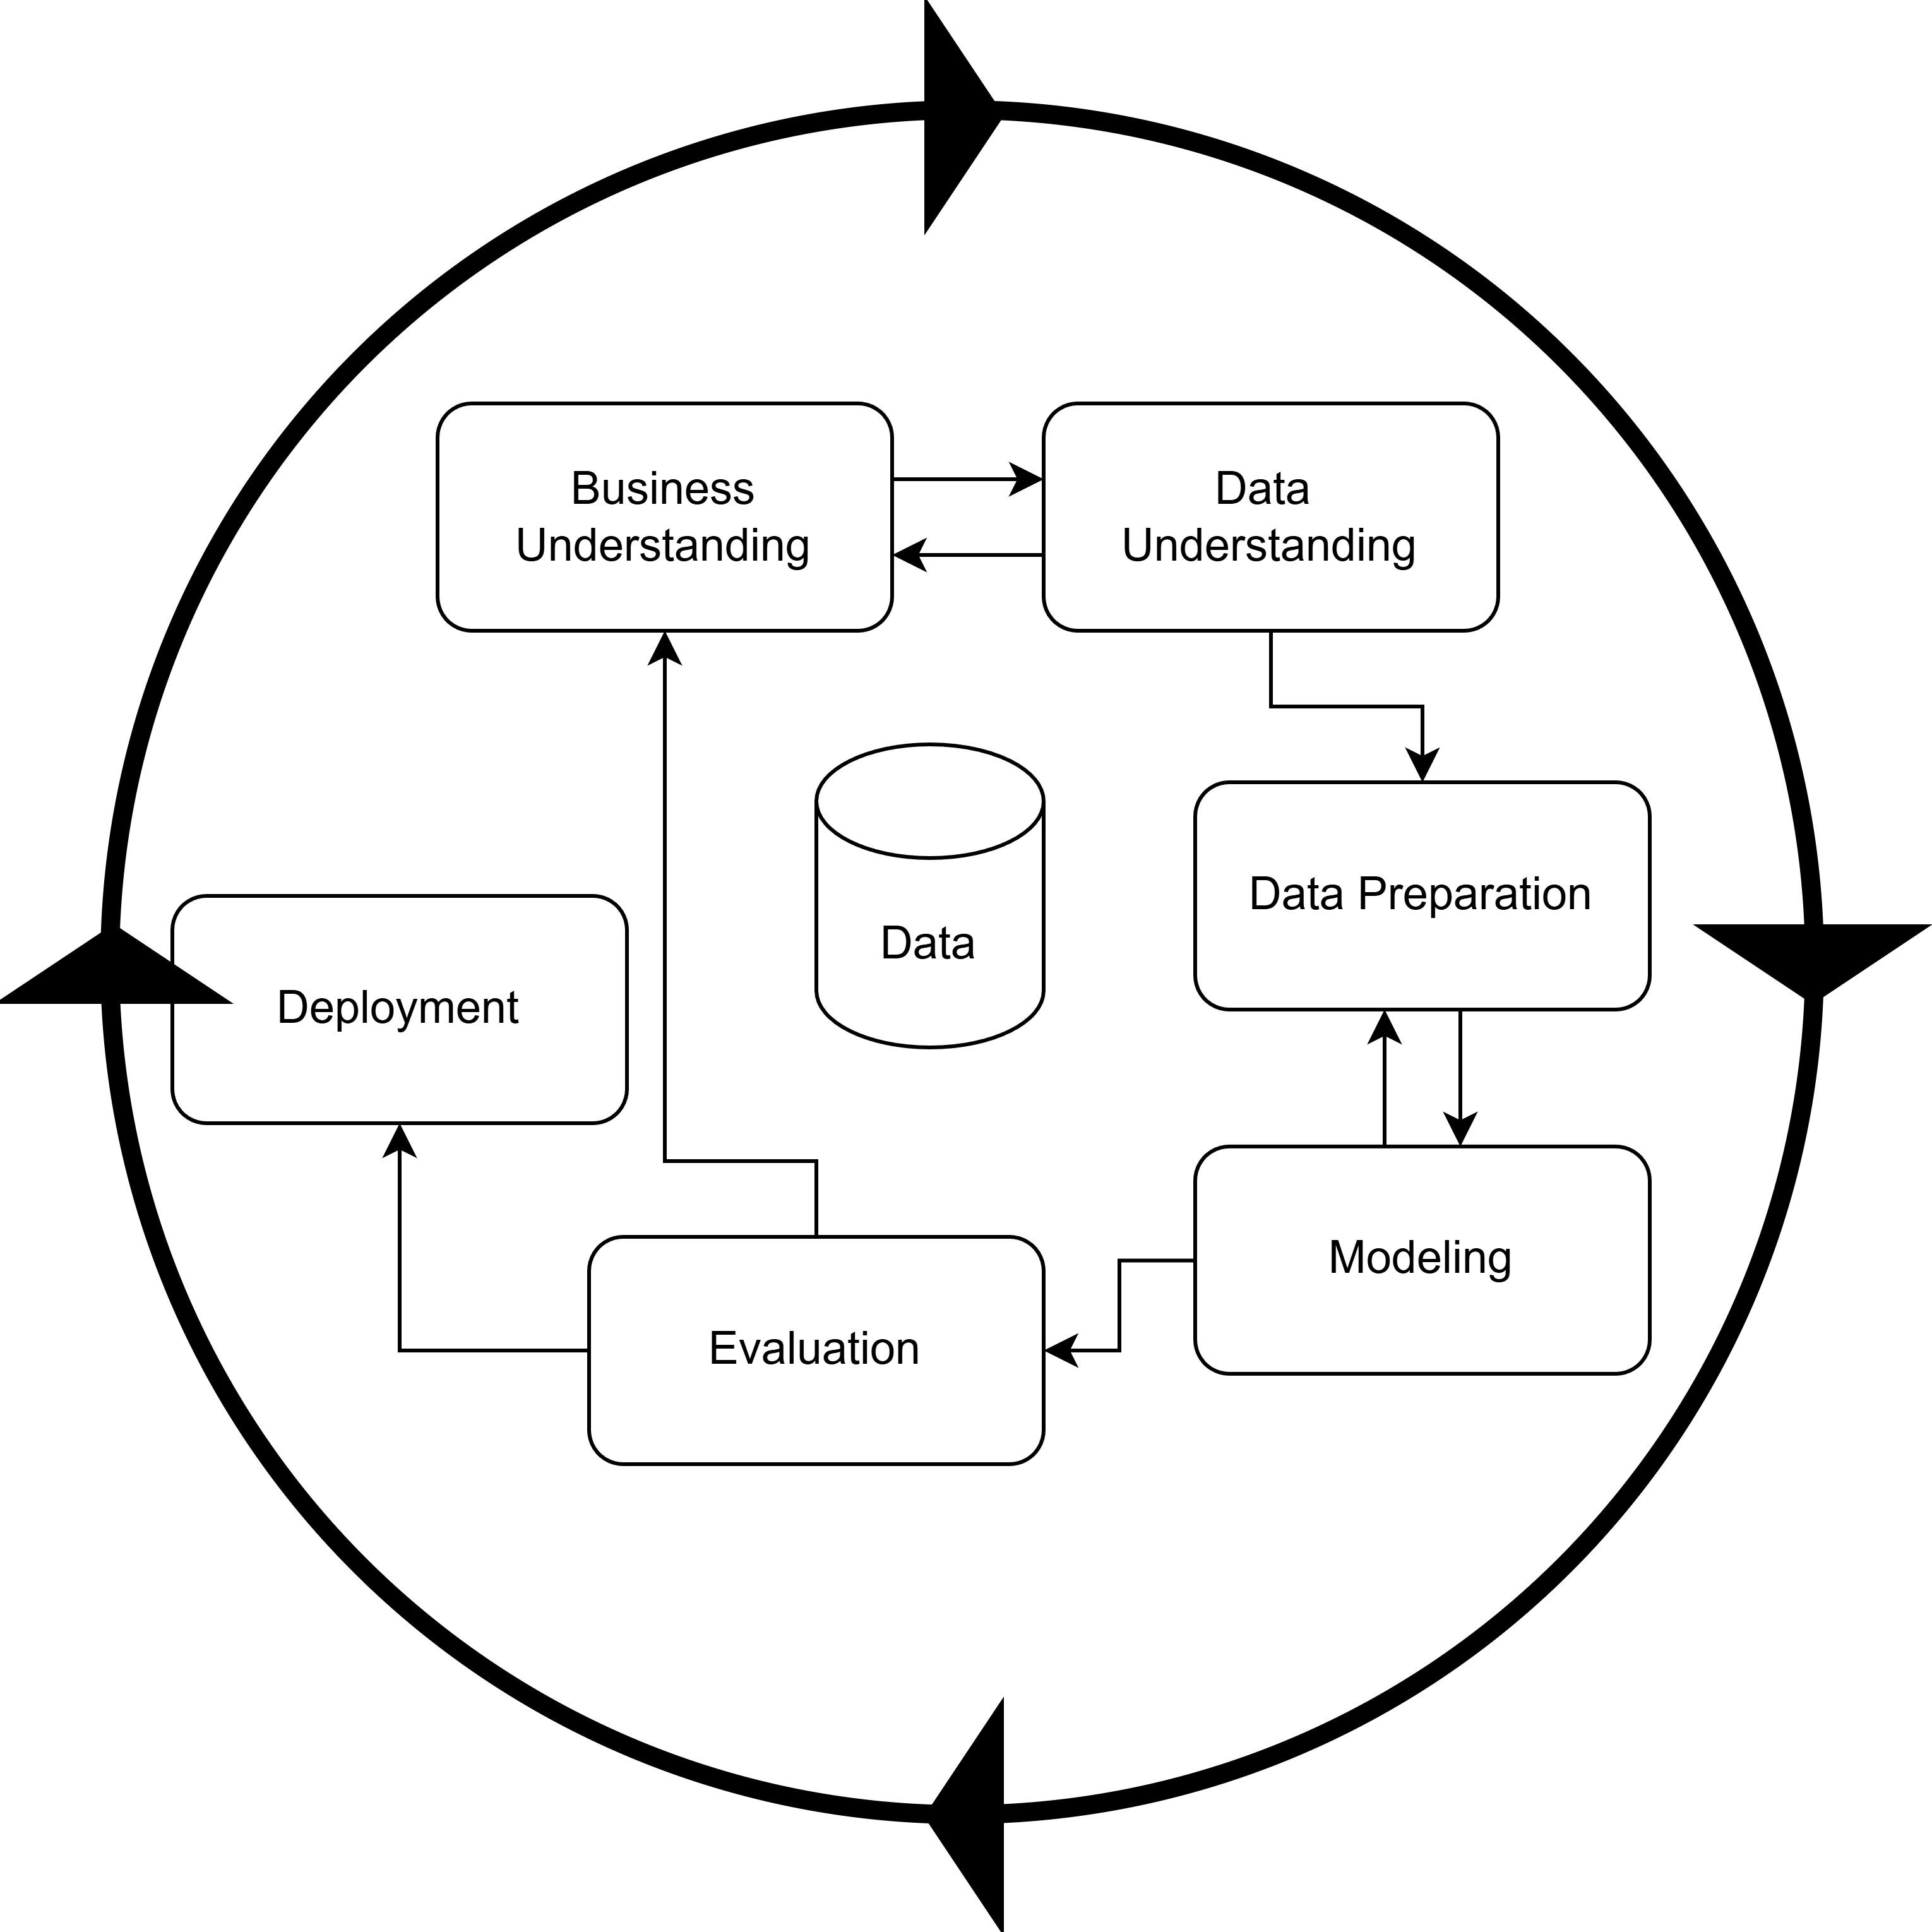
\includegraphics[width=0.7\textwidth]{images/CRISP-DM.png}
	\caption{\textit{Cross-Industry Process for Data Mining} (CRISP-DM) 
		\autocite{chapman2000crispdm}}
	\label{gambar:crispdm}
\end{figure}


Keseluruhan tahapan yang akan dilalui selama pelaksanaan tugas akhir, yang spesifik untuk menyelesaikan persoalan yang diangkat, adalah sebagai berikut.

\begin{enumerate}
	\item	\textit{Business Understanding}
	
	\textit{Business Understanding} dilakukan untuk mengidentifikasi permasalahan tumor otak yang terjadi di Indonesia dan potensi solusi yang dapat dihadirkan oleh kecerdasan buatan.
	Proses investigasi dan pengumpulan fakta pada tahap ini dilakukan melalui studi literatur sistematis. Pencarian literatur berfokus pada basis data akademik seperti Google Scholar, Scopus, dan SpringerLink, menggunakan kombinasi kata kunci seperti "tumor otak", "\textit{CT Scan}", "\textit{deep learning}", dan "XAI". \textit{Filtering} literatur dilakukan untuk mendapatkan sumber primer yang relevan dan terbaru sehingga menjamin validitas dan relevansi solusi yang diusulkan.
	Hal ini dilakukan dengan mencari studi literatur mengenai permasalahan tumor otak yang ada. Setelah itu, dilakukan pencarian solusi-solusi yang sudah berjalan dan yang sedang dikembangkan. Berdasarkan permasalahan dan solusi, dilakukan pendefinisian terhadap tujuan, persyaratan, dan rumusan masalah yang ingin dicapai.
	
	\item	\textit{Data Understanding}
	
	\textit{Data Understanding} dilakukan untuk mengenali dan memeriksa \textit{dataset} untuk mengidentifikasi karakteristik, kualitas, dan wawasan awal. Tahap ini dilakukan dengan mencari \textit{dataset} publik citra \textit{CT Scan} otak, lalu memeriksa data tersebut untuk mengetahui regulasi dalam pengumpulan data tersebut serta memeriksa kualitas data, seperti jumlah data dan distribusi kelas untuk mengidentifikasi potensi masalah dan hal yang harus dilakukan pada data tersebut.
	
	\item	\textit{Data Preparation}
	
	\textit{Data Preparation} bertujuan untuk menghasilkan data yang bersih dan sesuai dengan model yang ingin digunakan. \textit{Data Preparation} dilakukan dengan cara membagi data menjadi tiga bagian, yaitu data latih, validasi, dan uji. Setelah itu, dilakukan pembersihan data yang memiliki kualitas rendah atau data \textit{outlier}, \textit{preprocessing} pada citra, dan penyeragaman format data citra sesuai dengan model yang akan digunakan.
	
	\item	\textit{Modeling}
	
	\textit{Modeling} dilakukan untuk memilih dan menetapkan teknik pemodelan yang ingin dilakukan dan melatihnya menggunakan hasil dari \textit{Data Preparation}. \textit{Modeling} dilakukan dengan memilih arsitektur model dan teknik XAI yang akan digunakan, membangun model menggunakan data latih, mengatur \textit{hyperparameter} model untuk meningkatkan performa, dan menilai kinerja model-model yang telah dibuat untuk disimpan pada evaluasi.
	
	\item	\textit{Evaluation}
	
	\textit{Evaluation} dilakukan untuk memastikan model yang telah dipilih dapat mencapai tujuan penelitian dan menjawab rumusan masalah yang sudah dibuat. \textit{Evaluation} dilakukan dengan mengukur performa model CNN secara kuantitatif, seperti metrik akurasi, presisi, dan \textit{recall}, serta mengukur performa model XAI secara kuantitatif berdasarkan \textit{ground truth} untuk melihat seberapa signifikan XAI dapat menyoroti area tumor.
	
	
	\item	\textit{Deployment}
	
	Pada pengerjaan Tugas Akhir ini tidak dilakukan tahapan \textit{Deployment}.
	
\end{enumerate}

% Sistematika Penulisan
\section{Sistematika Penulisan}
Tuliskan gambaran umum isi dari setiap bab yang ada dalam laporan tugas akhir. Sistematika penulisan ini memberikan panduan bagi pembaca tentang struktur dan alur pembahasan dalam laporan tugas akhir. Berikut adalah contoh sistematika penulisan yang dapat diikuti:
\begin{enumerate}
	\item	Bab I Pendahuluan: Berisi latar belakang, rumusan masalah, tujuan, batasan masalah, metodologi, dan sistematika penulisan laporan tugas akhir.
	\item	Bab II Studi Literatur: Berisi kajian pustaka yang relevan dengan topik tugas akhir, termasuk teori-teori, konsep-konsep, dan hasil-hasil penelitian sebelumnya yang mendukung pelaksanaan tugas akhir.
	\item	Bab III Analisis: Berisi penjelasan tentang analisis masalah dan kebutuhan pengguna serta berbagai alternatif solusinya.
	\item   Bab IV Perancangan: Berisi penjelasan tentang perancangan solusi yang diusulkan, yaitu \textit{dataset} yang akan digunakan, \textit{preprocessing} dari data tersebut, perancangan model, dan perancangan evaluasi yang akan dilakukan.
	\item	Bab V Implementasi: Berisi penjelasan tentang proses implementasi solusi yang diusulkan, termasuk langkah-langkah yang diambil dan hasil yang diperoleh.
	\item	Bab VI Evaluasi: Berisi analisis dan evaluasi terhadap solusi yang diimplementasikan, termasuk metode pengujian, hasil pengujian, dan penilaian kinerja.
	\item   Bab VII Kesimpulan dan Saran: Berisi kesimpulan dari hasil pelaksanaan tugas akhir dan saran untuk pengembangan lebih lanjut.
	\item   Daftar Pustaka: Berisi daftar referensi yang digunakan dalam penyusunan laporan tugas akhir.
	\item   Lampiran: Berisi dokumen-dokumen pendukung seperti kode program.
\end{enumerate}